%(BEGIN_QUESTION)
% Copyright 2015, Tony R. Kuphaldt, released under the Creative Commons Attribution License (v 1.0)
% This means you may do almost anything with this work of mine, so long as you give me proper credit

Beregn strømmen gjennom $R_4$ i denne serie-parallell-kretsen, samt spenningen mellom punktene B og D. Du trenger ikke å oppgi strømretning eller spenningspolaritet. Anta at alle motstandene har verdien 1 k$\Omega$:

$$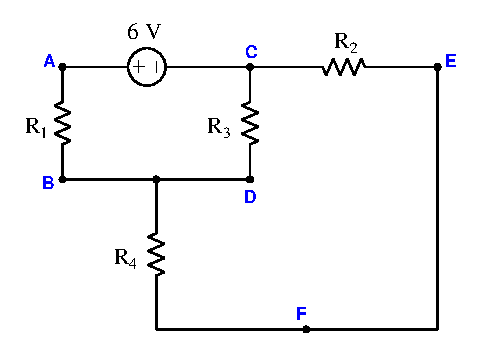
\includegraphics[width=15.5cm]{i00319x01.eps}$$

$I_{R4}$ = 

\vskip 10pt

$V_{BD}$ = 

\vskip 10pt

\underbar{file i00319}
%(END_QUESTION)





%(BEGIN_ANSWER)

$I_{R4}$ = 1.2 mA

\vskip 10pt

$V_{BD}$ = 0 V

%(END_ANSWER)





%(BEGIN_NOTES)

{\bf Denne oppgaven er ment for eksamen og ikke for arbeidsark!}.

%(END_NOTES)
